\documentclass{article}
\usepackage[utf8]{inputenc}
\usepackage[english]{babel}
\usepackage[T1]{fontenc}

\usepackage{amsfonts}
\usepackage{amsmath}
\usepackage{amssymb}
\usepackage{tikz}
\usepackage{graphicx}
\usepackage{color}
\usepackage{enumitem}
\usetikzlibrary{arrows}
\usepackage{framed}
\usepackage{arydshln}
\usepackage{multirow}


% no indent
\setlength\parindent{0pt}

% commands
\usepackage{amsthm}
\theoremstyle{definition}
\newtheorem{definition}{Definition}[section]

\newcommand{\domain}{\mathcal{D}}
\newcommand{\image}{\mathcal{I}}
\newcommand{\real}{\mathbb{R}}

\newcommand{\todo}[1]{\textcolor{red}{TODO: #1}}




\title{Structures en apprentissage profond.\\ On structures in deep learning}

\begin{document}

\section{Definitions}

\subsection{Deep learning}

\todo{}

\subsection{Graphs}

A graph $G$ is defined as a couple $(V,E)$ where $V$ represents the set of nodes and $E \subseteq\binom{V}{2}$ is the set of edges connecting these nodes.

\todo{Example of figure}

We encounter the notion of graphs several times in deep learning:
\begin{itemize}
\item Connections between two layers of a deep learning model can be represented as a bipartite graph, coined \emph{connectivity graph}. It encodes how the information is propagated through a layer to another. See section~\ref{con_graph}.
\item A computation graph is used by deep learning frameworks to keep track of the dependencies between layers of a deep learning models, in order to compute forward and back-propagation. See section~\ref{comp_graph}.
\item A graph can represent the underlying structure of an object (often a vector), whose nodes represent its features. See section~\ref{inductive_graph}.
\item Datasets can also be graph-structured, where the nodes represent the objects of the dataset. See section~\ref{transductive_graph}.
\end{itemize}

\subsubsection{Connectivity graph}
\label{con_graph}

A Connectivity graph is a graphical representation of the linear part of the mathematical model implemented by a layer of neurons.
%$U = \{u_1, u_2, \ldots, u_n\}$
Formally, given a linear part of a layer, let $\textbf{x}$ and $\textbf{y}$ be the input and output signals, $n$ the size of the set of input neurons $N = \{u_1, u_2, \ldots, u_n\}$, and $m$ the size of the set of output neurons $M = \{v_1, v_2, \ldots, v_m\}$. This layer implements the equation $y = \Theta x$ where $\Theta$ is a $n \times m$ matrix.

\begin{definition}
{The \emph{connectivity graph} $G = (V,E)$ is defined such that $V = N \cup M$ and $E = \{(u_i,v_j) \in  N \times M, \Theta_{ij} \neq 0 \} $.}
\end{definition}

I.e. the connectivity graph is obtained by drawing an edge between neurons for which $\Theta_{ij} \neq 0$.
For instance, in the special case of a complete bipartite graph, we would obtain a dense layer. 
Connectivity graphs are especially useful to represent partially connected layers, for which most of the $\Theta_{ij}$ are $0$. 
For example, in the case of layers characterized by a small local receptive field, the connectivity graph would be sparse, and output neurons would be connected to a set of input neurons that corresponds to features that are close together in the input space. Figure~\ref{con_ex} depicts some examples.

\begin{figure}[h]
  \begin{center}
    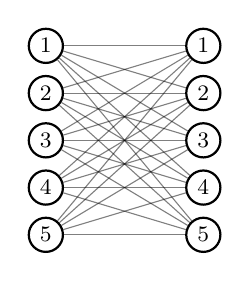
\begin{tikzpicture}
      \tikzstyle{every node} = [draw, circle, thick, inner sep = 2pt]
      \foreach \y in {0,...,4}{
        \pgfmathtruncatemacro{\yplusone}{5 - \y}
        \node(a\y) at (0,.6*\y) {\footnotesize\yplusone};
      }
      \foreach \y in {0,...,4}{
        \pgfmathtruncatemacro{\yplusone}{5 - \y}
        \node(\y) at (2,.6*\y) {\footnotesize\yplusone};
      }

      \foreach \x in {0,...,4}{
        \foreach \y in {0,...,4}{
          \path[opacity=0.5] (a\x) edge (\y);
        }
      }
    \end{tikzpicture}
  \end{center}
  \caption{Examples}
  \label{con_ex}
\end{figure}

\todo{Figure~\ref{con_ex}. It's just a placeholder right now}


Connectivity graphs also allow to graphically modelize how weights are tied in a neural layer. Let's suppose the $\Theta_ij$ are taking their values only into the finite set $K = \{w_1, w_2, \ldots, w_\kappa\}$ of size $\kappa$, which we will refer to as the \emph{kernel} of \emph{weights}. Then we can define a labelling of the edges $s: E \rightarrow K$. $s$ is called the \emph{weight sharing scheme} of the layer. This layer can then be formulated as $\displaystyle \forall v \in M, y_v = \sum_{u \in N, (u,v) \in E} w_{s(u,v)} x_u$. Figure~\ref{cnn} depicts the connectivity graph of a 1-d convolution layer and its weight sharing scheme.

\begin{figure}[h]
  \begin{center}
    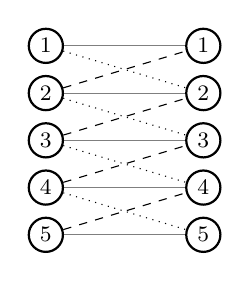
\begin{tikzpicture}
      \tikzstyle{every node} = [draw, circle, thick, inner sep = 2pt]
      \foreach \y in {0,...,4}{
        \pgfmathtruncatemacro{\yplusone}{5 - \y}
        \node(a\y) at (0,.6*\y) {\footnotesize\yplusone};
      }
      \foreach \y in {0,...,4}{
        \pgfmathtruncatemacro{\yplusone}{5 - \y}
        \node(\y) at (2,.6*\y) {\footnotesize\yplusone};
      }
      \path[opacity=0.5]
      (a0) edge (0);
      \path[dashed]
      (a0) edge (1);
      \path[dotted]
      (a1) edge (0);
      \path[opacity=0.5]
      (a1) edge (1);
      \path[dashed]
      (a1) edge (2);
      \path[dotted]
      (a2) edge (1);
      \path[opacity=0.5]
      (a2) edge (2);
      \path[dashed]
      (a2) edge (3);
      \path[dotted]
      (a3) edge (2);
      \path[opacity=0.5]
      (a3) edge (3);
      \path[dashed]
      (a3) edge (4);
      \path[dotted]
      (a4) edge (3);
      \path[opacity=0.5]
      (a4) edge (4);
    \end{tikzpicture}
  \end{center}
  \caption{Depiction of a 1D-convolutional layer and its weight sharing scheme.}
  \label{cnn}
\end{figure}


\todo{Add weight sharing scheme in Figure~\ref{cnn}}

\subsubsection{Computation graph}
\label{comp_graph}

\subsubsection{Underlying graph structure}
\label{inductive_graph}

\subsubsection{Graph-structured dataset}
\label{transductive_graph}

transductive vs inductive

\subsection{Geometric grids}

\subsection{Grid graphs}

\subsection{Spatial graphs}

\subsection{Projections of spatial graphs}

\end{document}